\documentclass[12pt]{report}
\usepackage[a4paper, left=3.17cm, right=3.17cm, top=2.54cm, bottom=2.54cm]{geometry}
\usepackage[T1]{fontenc}
\usepackage{mathptmx}
\usepackage{amsmath}
\usepackage{amsfonts}
\usepackage{chemformula}
\usepackage{multicol}
\usepackage{multirow}
\usepackage{tabularx,booktabs}
\newcolumntype{C}{>{\centering\arraybackslash}X} % centered version of "X" type
\usepackage[linesnumbered,ruled,vlined]{algorithm2e}
\usepackage{comment}
\usepackage{array}
\newcolumntype{P}[1]{>{\centering\arraybackslash}p{#1}}
\usepackage{cite}
\usepackage[colorlinks, linkcolor=black, anchorcolor=black, citecolor=black]{hyperref}
\usepackage{graphicx}
\setlength{\parskip}{0.5em}
\title{Path-finding in Maze using different Algorithm and Comparisons }
%\author{\textup{Qi YUAN}}


%copyright at footer
\usepackage{fancyhdr}
\fancyhf{}
\rfoot{%
  \footnotesize
  \textcopyright~Dept. of Computer Science and Engineering, GUB\\

 }
%\pagestyle{fancy}


\usepackage{listings}
\usepackage{color}

\definecolor{dkgreen}{rgb}{0,0.6,0}
\definecolor{gray}{rgb}{0.5,0.5,0.5}
\definecolor{mauve}{rgb}{0.58,0,0.82}

\lstset{frame=tb,
  language=Java,
  aboveskip=3mm,
  belowskip=3mm,
  showstringspaces=false,
  columns=flexible,
  basicstyle={\small\ttfamily},
  numbers=none,
  numberstyle=\tiny\color{gray},
  keywordstyle=\color{blue},
  commentstyle=\color{dkgreen},
  stringstyle=\color{mauve},
  breaklines=true,
  breakatwhitespace=true,
  tabsize=3
}











\begin{document}
    \begin{titlepage}
\center 
\newcommand{\HRule}{\rule{\linewidth}{0.1mm}}

\includegraphics[scale=0.6]{Figures/GUB.png}\\[1cm] 
\center 
%\quad\\[1.5cm]
\textsl{\Large Green University of Bangladesh }\\[0.5cm] 
\textsl{\large Department of Computer Science and Engineering (CSE)}\\
%\textsl{\large Faculty of Sciences and Engineering (FSE)}\\
\textsl{\large Semester: (Fall, Year: 2022), B.Sc. in CSE (Day)}\\[0.5cm] 
\makeatletter
\HRule \\[0.4cm]
{ \huge \bfseries \@title}\\[0.2cm] 
\HRule \\[1.0cm]

\textsl{\large Course Title: Algorithms Lab }\\
\textsl{\large Course Code: CSE 206}\\ 
\textsl{\large Section: 221 - D9}\\[0.5cm] 

{\large \underline{Students Details}}\\[0.2cm]

\begin{table*}[htb]
\centering
\begin{tabular}{ |P{7.0cm}|P{3.5cm}|}
\hline
\textbf{Name} & \textbf{ID}\\
\hline
Jahidul Islalm  & 221002504 \\
\hline
- & - \\
\hline
\end{tabular}
\end{table*}
\vspace{0.5cm}


\textsl{\large Submission Date: \ 01/01/2024 }\\ 
\textsl{\large Course Teacher’s Name: \ Md. Abu Rumman Refat  }\\[0.9cm] 




\makeatother
{\large [For teachers use only: \textcolor{red}{Don’t write anything inside this box]}}\\

\begin{table}[]
\centering
\begin{tabular}{|p{7.5cm}p{7.0cm}|}
\hline
\multicolumn{2}{|c|}{{\underline{\textbf{Lab Project Status}}}} \\
 & \\\hline
\textbf{Marks:}                & \textbf{Signature:}        \\
 & \\ 
\textbf{Comments:}             & \textbf{Date:}             \\ 
 & \\\hline
\end{tabular}
\end{table}


\end{titlepage}


    \tableofcontents
  


% Chapter 1 starting here.....    
\newpage
\chapter{Introduction}

\section{Overview}
The problem of pathfinding in a maze is a classic and fundamental topic in computer science and artificial intelligence. It involves finding the most efficient route from a designated start point to a specified end point within a maze, which is typically represented as a grid with obstacles and open paths. This problem has wide-ranging applications in various domains, including robotics, video games, network routing, and logistics, where efficient navigation is crucial.

\section{Motivation}
The motivation behind studying pathfinding in a maze lies in its real-world applicability and the need for efficient solutions to navigate complex environments. As technology advances, the demand for intelligent systems capable of autonomously finding optimal paths becomes increasingly prevalent. From guiding robots through cluttered spaces to enhancing user experiences in video games, the ability to solve maze navigation problems is integral to the development of intelligent and adaptive systems. \cite{farokhzad2009impact}.

\section{Problem Definition}

\subsection{Problem Statement}
The problem can be formally defined as follows: Given a maze represented as a grid with specified start ('S') and end ('E') points, along with obstacles represented by '#' and open paths denoted by '.', the task is to determine the shortest path from the start to the end while avoiding obstacles. Various algorithms can be employed to solve this problem, each with its own set of strengths and weaknesses.

\subsection{Complex Engineering Problem}
Table \ref{tab:CEP}
The pathfinding problem in a maze is a complex engineering challenge that encompasses several key aspects:


\begin{table}[htbp]
   \centering
    \caption{Summary of the attributes touched by the mentioned projects}
    \begin{tabular}{|p{6.0 cm}|p{8 cm}|}
    %\rowcolor{gray!30}
    \toprule
        \textbf{Name of the P Attributess} & \textbf{Explain how to address}  \\
        \midrule

    \textbf{P1:} Depth of knowledge required  &  -Employed a systems engineering approach to identify, prioritize, and manage conflicting requirements. Utilized techniques such as requirement traceability matrices and trade-off analyses to balance conflicting demands. Clearly defined design constraints and use decision support tools to optimize the trade-offs. \\
      \hline
       
    \textbf{P2:} Range of conflicting
     requirements  &  ---- \\
      \hline

    \textbf{P3:} Depth of analysis required  &  Undertook a detailed analysis of the problem, considering the complexities introduced by different maze structures, algorithmic choices, and user interactions. Use algorithmic analysis to evaluate the time and space complexity of pathfinding algorithms. Performed sensitivity analyses to understand the impact of parameter variations. \\
    \hline
    
    \textbf{P4:} Familiarity of issues  &  Conducted a thorough review of existing solutions, best practices, and common challenges related to pathfinding in mazes. Engaged with the relevant literature and case studies to gain insights into common issues and successful strategies. \\ 
    \hline
    \textbf{P5:} Extent of applicable codes  &  ---- \\
      \hline
       
    \textbf{P6:} Extent of stakeholder
     involvement and conflicting
     requirements  &  ---- \\
      \hline

    \textbf{P7:} Interdependence  &  ---- \\
    \hline
        
    \end{tabular}
    \label{tab:CEP}
\end{table}

\section{Design Goals/Objectives}
The primary objective of this project is to implement and analyze different pathfinding algorithms to find the optimal solution to the maze navigation problem. The project encompasses the design and implementation of user-friendly interfaces, incorporation of multiple maze generation algorithms, inclusion of various pathfinding algorithms (such as Breadth-First Search, Depth-First Search, Dijkstra's Algorithm, and A*), and the provision of features allowing users to customize and compare algorithmic performances. The project aims to provide an educational and interactive platform for users to explore the intricacies of pathfinding algorithms.

\section{Application}
The applications of pathfinding in a maze are diverse and impact several key domains, showcasing its significance in various real-world scenarios:



\subsection{Robotics and Autonomous Vehicles: }
Pathfinding algorithms are crucial for guiding robots and autonomous vehicles through complex environments, ensuring safe and efficient navigation in both industrial and public spaces.\\
\subsection{Video Games and Virtual Environments:}
In the realm of entertainment and simulations, pathfinding plays a vital role in creating lifelike and intelligent behaviors for characters and entities. This is essential for designing engaging and challenging gameplay experiences.\\
\subsection{Network Routing and Traffic Management: }
Pathfinding algorithms contribute to the optimization of network routes, aiding in efficient data transmission and traffic management in communication networks and the internet. This is particularly relevant in the context of data centers and routing protocols.\\
\subsection{Logistics and Supply Chain Optimization: }
The logistics industry relies on pathfinding to optimize delivery routes, reduce transportation costs, and enhance overall supply chain efficiency. It helps in determining the most cost-effective and timely paths for goods and services.\\


\subsection{Urban Planning and Infrastructure Design:}
City planners use pathfinding techniques to analyze pedestrian and vehicular movement, contributing to the design of efficient transportation systems, public spaces, and infrastructure layouts.\\

 
\subsection{Routing in Geographic Information Systems (GIS): }
Geographic information systems leverage pathfinding algorithms for routing applications, guiding users through maps, suggesting optimal routes for navigation, and facilitating location-based services.\\
 
\subsection{Artificial Intelligence and Decision Support Systems: }
Pathfinding algorithms are integral components of decision support systems and AI applications, aiding in intelligent decision-making processes across diverse domains, including finance, healthcare, and resource allocation.\\

\subsection{Educational Tools and Simulations: }
Pathfinding in mazes serves as a valuable educational tool, allowing students and enthusiasts to explore and understand the principles of algorithmic navigation in a visually intuitive manner.\\

By addressing the maze pathfinding problem, we not only tackle fundamental challenges in computer science but also contribute to the development of solutions that impact the efficiency and intelligence of systems across a wide range of applications, ultimately enhancing our technological landscape.
In every section please add subsections and figures and citations as references\cite{farokhzad2009impact} also.

% Chapter 1 ends here.....    




% Chapter 2 starting here.....    
\newpage
\chapter{Implementation of the Project}

\section{Introduction}
This chapter delves into the development and implementation of a maze-solving project employing various algorithms. The project aims to devise efficient algorithms to find paths from the start to the end in a maze. Three distinct algorithms, namely Breadth-First Search (BFS), Depth-First Search (DFS), and A* (A-star), are explored and implemented to address this classic problem. This chapter provides an overview of the project's goals, algorithm selection, programming language, project components, and a summary of the implemented solutions.  \cite{9134044} \cite{DFS} \cite{A*}. 

\section{Project Details}
The project addresses the maze-solving problem, wherein algorithms are tasked with navigating through a maze from a designated start point  'S'  to an endpoint 'E' . The maze consists of open paths '.', walls  '#' , and the algorithms must find solutions that traverse the open paths while avoiding the walls.
\section{Algorithm Selection}
Three algorithms have been chosen to tackle the maze-solving problem, each with its unique approach:

\begin{figure}[h]
        \begin{center}
         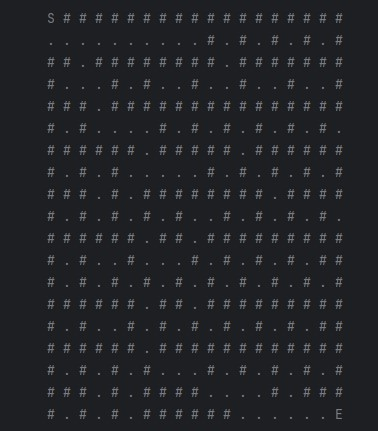
\includegraphics[width=1\linewidth]{Figures/grid.jpg}
        \end{center}
        \caption{A Sample Maze}
     \end{figure}

\subsection{Breadth-First Search (BFS)}
BFS explores the maze level by level, considering all neighbors at the current depth before moving on to the next depth. This algorithm ensures the shortest path is found.

\subsection{Depth-First Search (DFS)}
DFS explores the maze by going as deep as possible along each branch before backtracking. While not guaranteed to find the shortest path, DFS is often more memory-efficient and can uncover multiple solutions.
\subsection{A* Algorithm}
A* is a heuristic-based algorithm that combines elements of Dijkstra's algorithm and greedy best-first search. It uses heuristics to guide the search toward the most promising paths, providing an efficient and optimal solution.



\section{Implementation}
The project is implemented in Java, a versatile and widely-used programming language known for its readability, portability, and object-oriented features. Java provides a robust foundation for implementing complex algorithms and data structures, making it an ideal choice for this maze-solving endeavor.



\subsection{Breadth-First Search (BFS)}
\subsubsection{solveMazeBFS Method:}

\begin{itemize}
    \item This method takes the maze and the starting position as input and returns a boolean indicating whether a path from the start to the end is found using BFS.
\end{itemize}

\begin{itemize}
    \item It uses a queue (LinkedList in this case) to keep track of positions to be explored in a breadth-first manner.
\end{itemize}

\begin{itemize}
    \item A boolean array visited is used to mark visited positions to avoid revisiting them.
\end{itemize}



\subsubsection{BFS Algorithm:}

\begin{itemize}
    \item The BFS algorithm starts from the initial position and explores all valid neighboring positions before moving on to the next level.
\end{itemize}

\begin{itemize}
    \item It continues this process until the end position is reached or all possible paths have been explored.
\end{itemize}

\begin{itemize}
    \item The directions array represents possible movements (up, down, left, right).
\end{itemize}


\subsubsection{Main Method:}

\begin{itemize}
    \item In the main method, a sample maze is defined, and the solveMazeBFS function is called with the starting position obtained using findStart.
\end{itemize}

\begin{itemize}
    \item Depending on whether a path is found or not, an appropriate message is printed.
\end{itemize}





\subsection{Dept-First Search (DFS)}
\subsubsection{Main Method:}

\begin{itemize}
    \item A 2D char array (maze) represents the maze, where 'S' denotes the start, 'E' denotes the end, '#' denotes walls, and '.' denotes open paths.
\end{itemize}

\begin{itemize}
    \item The solveMaze method is called with the maze and the starting position obtained using findStart.
\end{itemize}

\begin{itemize}
    \item Depending on whether a path is found or not, an appropriate message is printed, and the final state of the maze is displayed using printMaze.
\end{itemize}



\subsubsection{solveMaze Method:}

\begin{itemize}
    \item It acts as a wrapper for the actual recursive backtracking method, recursiveBacktracker.
\end{itemize}

\begin{itemize}
    \item It returns true if a path from the start to the end is found, otherwise false.
\end{itemize}

\begin{itemize}
    \item The directions array represents possible movements (up, down, left, right).
\end{itemize}


\subsubsection{recursiveBacktracker Method:}

\begin{itemize}
    \item This method performs the actual DFS traversal to explore paths in the maze.
\end{itemize}

\begin{itemize}
    \item It recursively checks and explores in all directions (up, down, left, right) until it finds the end or determines that no path exists.
\end{itemize}
\begin{itemize}
    \item It marks visited positions as 'V' and backtracks if necessary.
\end{itemize}

\subsubsection{findStart Method:}

\begin{itemize}
    \item It searches for the starting position 'S' in the maze and returns its coordinates as an array.
\end{itemize}
\subsubsection{printMaze Method:}

\begin{itemize}
    \item It prints the current state of the maze to the console.
\end{itemize}







\subsection{A* Algorithm}
\subsubsection{Main Method:}

\begin{itemize}
    \item Defines a maze represented by a 2D character array.
\end{itemize}

\begin{itemize}
    \item Defines a maze represented by a 2D character array.
\end{itemize}

\begin{itemize}
    \item Prints whether a path is found and, if so, prints the maze with the path marked.
\end{itemize}



\subsubsection{solveMazeAStar Method}

\begin{itemize}
    \item Implements the A* algorithm to find the shortest path in the maze.
\end{itemize}

\begin{itemize}
    \item Uses a priority queue (PriorityQueue<Node> pq) to prioritize nodes with lower total cost.
\end{itemize}

\begin{itemize}
    \item Explores neighboring nodes, considering both the actual cost and the heuristic estimate.
\end{itemize}
\begin{itemize}
    \item Reconstructs and marks the path in the maze if the end is reached.
\end{itemize}


\subsubsection{isValid Method}

\begin{itemize}
    \item Checks if a given position is within the bounds of the maze.
\end{itemize}

\subsubsection{findStart Method}

\begin{itemize}
    \item Finds the starting position ('S') in the maze.
\end{itemize}

\subsubsection{heuristic Method}

\begin{itemize}
    \item Implements a simple Manhattan distance heuristic.
\end{itemize}

\subsubsection{Node Classd}

\begin{itemize}
    \item Represents a node in the A* algorithm, storing information such as position, cost, heuristic value, and parent node.
\end{itemize}




















\section{Algorithms}
The algorithms breadth-first search (BFS) algorithm and the programming codes in detail should be included .\\Pseudo-codes are also encouraged very much to be included in this chapter for your project.

\begin{itemize}
    \item Breadth-First Search Algorithm
\end{itemize}





\begin{document}

\begin{algorithm}[H]
\DontPrintSemicolon
  
  \KwInput{Graph $G$, Source node $s$}
  \KwOutput{Visited nodes}
  \KwData{Queue $Q$}
  
  \tcc{Initialization}
  \For{each node $v$ in $G$}{
    Mark $v$ as not visited\;
  }
  Enqueue $s$ into $Q$ \tcp*{Enqueue the source node}
  Mark $s$ as visited\;
  
  \tcc{BFS traversal}
  \While{$Q$ is not empty}{
    Dequeue a node $u$ from $Q$\;
    Visit $u$ \tcp*{Process the current node}
    
    \For{each neighbor $v$ of $u$}{
      \If{$v$ is not visited}{
        Mark $v$ as visited\;
        Enqueue $v$ into $Q$\;
      }
    }
  }
  
  \caption{Breadth-First Search Algorithm}
\end{algorithm}

\\
\begin{itemize}
    \item Depth-First Search Algorithm
\end{itemize}

\begin{document}

\begin{algorithm}[H]
\DontPrintSemicolon
  
  \KwInput{Graph $G$, Source node $s$}
  \KwOutput{Visited nodes}
  \KwData{Stack $S$}
  
  \tcc{Initialization}
  \For{each node $v$ in $G$}{
    Mark $v$ as not visited\;
  }
  Push $s$ onto $S$ \tcp*{Push the source node onto the stack}
  
  \tcc{DFS traversal}
  \While{$S$ is not empty}{
    Pop a node $u$ from $S$\;
    \If{$u$ is not visited}{
      Visit $u$ \tcp*{Process the current node}
      Mark $u$ as visited\;
      
      \For{each neighbor $v$ of $u$}{
        \If{$v$ is not visited}{
          Push $v$ onto $S$ \tcp*{Push unvisited neighbors onto the stack}
        }
      }
    }
  }
  
  \caption{Depth-First Search Algorithm}
\end{algorithm}










% Chapter 2 ends here..... 








% Chapter 3 starting here..... 
\newpage
\chapter{Performance Evaluation}

\section{Simulation Environment/ Simulation Procedure}

For the performance evaluation of the Breadth-First Search (BFS) and Depth-First Search (DFS) algorithms, we utilized a simulation environment implemented in [Programming Language] on a [hardware specification]. The simulations were conducted on a [mention any specific software or tools used].

\subsection{BFS Simulation Environment}
Describe the specific configurations, software versions, and any dependencies needed for simulating the BFS algorithm. Include details about the maze representation and how the BFS algorithm interacts with it.

\subsection{DFS Simulation Environment}
Similarly, detail the simulation environment for the DFS algorithm, including configurations, software versions, and any dependencies. Provide information on how the maze is represented and how the DFS algorithm interacts with it.

\section{Results Analysis/Testing}

Our performance evaluation involved several aspects, including runtime efficiency, pathfinding accuracy, and scalability. Each algorithm was tested on various maze configurations to analyze its behavior in different scenarios.

\subsection{BFS Results Analysis}

\subsubsection{Result\_portion\_1}
The results of the BFS algorithm were obtained through simulations on different maze sizes. Screenshots and graphs, such as Figure \ref{fig:bfs-graph}, depict the algorithm's performance.



\subsubsection{Result\_portion\_2}
In this section, we present specific results related to the accuracy of the pathfinding by the BFS algorithm. Screenshots illustrating the optimal paths found in different mazes are included.

\begin{figure}[thbp]
    \begin{center}
        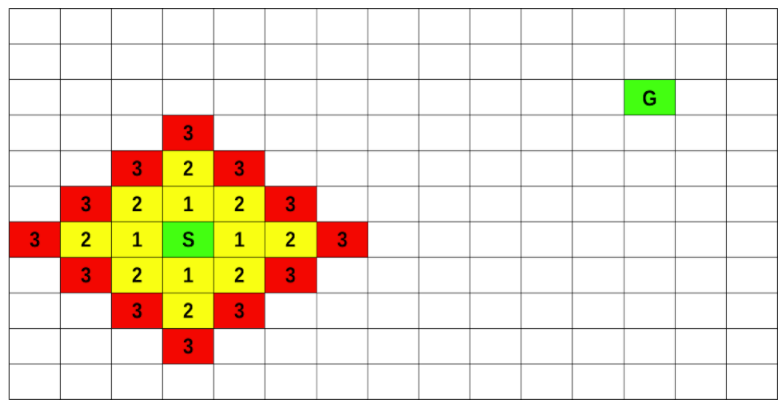
\includegraphics[width=0.5\textwidth]{Figures/image.png}
    \end{center}
    \caption{Optimal Path Found by BFS Algorithm}
\end{figure}

\subsubsection{Result\_portion\_3}
Discuss the implications of the results, any observed patterns, and potential improvements. Include a brief analysis of how the BFS algorithm performed in various scenarios.

\subsection{DFS Results Analysis}

\subsubsection{Result\_portion\_1}
Similar to the BFS section, provide specific results obtained from simulations of the DFS algorithm, including runtime graphs and screenshots (Figure \ref{fig:dfs-graph}).

\begin{figure}[thbp]
    \begin{center}
        \includegraphics[width=0.5\textwidth]{Figures/dfs-runtime-graph.png}
    \end{center}
    \caption{DFS Algorithm Runtime on Various Maze Sizes}
    \label{fig:dfs-graph}
\end{figure}

\subsubsection{Result\_portion\_2}
Present results related to the accuracy of pathfinding by the DFS algorithm. Screenshots illustrating the paths found in different mazes can be included.

\begin{figure}[thbp]
    \begin{center}
        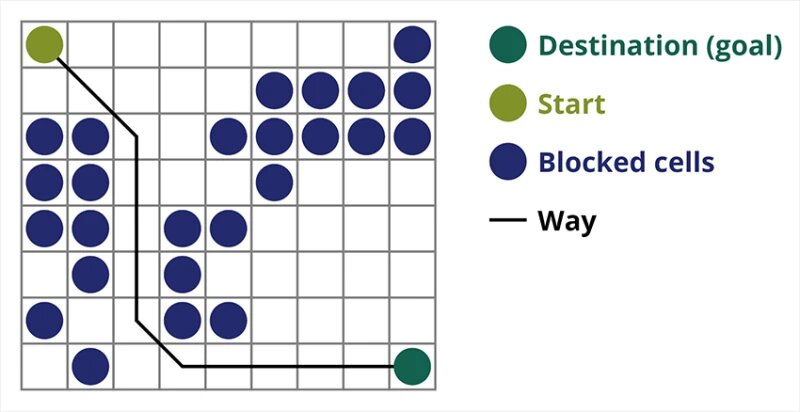
\includegraphics[width=0.5\textwidth]{Figures/Path.jpg}
    \end{center}
    \caption{Path Found by DFS Algorithm}
\end{figure}

\subsubsection{Result\_portion\_3}
Discuss the implications of the results, any observed patterns, and potential improvements. Include a brief analysis of how the DFS algorithm performed in various scenarios.

\section{Results Overall Discussion}

The overall performance of both BFS and DFS algorithms is discussed in this section, addressing their strengths, weaknesses, and how they compare in terms of runtime efficiency and pathfinding accuracy.

\subsection{BFS vs. DFS Comparison}
Provide a comprehensive comparison between BFS and DFS, considering factors such as computational complexity, scalability, and suitability for different types of mazes.






% Chapter 3 ends here..... 




% Chapter 5 starts here..... 
\newpage
\chapter{Conclusion}

\section{Conclusion}

In conclusion, the performance evaluation of the Breadth-First Search (BFS) and Depth-First Search (DFS) algorithms in maze-solving has provided valuable insights into their strengths and limitations. While both algorithms exhibit distinct characteristics, it is crucial to acknowledge certain limitations encountered during the project.

\subsection{BFS Limitations}

The BFS algorithm, known for its optimality in finding the shortest path, does have limitations, particularly concerning scalability. As the maze size increases, BFS may experience challenges due to its memory-intensive nature. The algorithm explores all possible paths level by level, and in larger mazes, the memory requirements can grow significantly. This may result in increased execution times and, in extreme cases, lead to resource exhaustion.

Moreover, BFS may struggle with mazes that have intricate structures or dead-end pathways. In scenarios where the optimal path involves navigating through convoluted passages, BFS might explore a large number of nodes before finding the solution, impacting its overall efficiency.

\subsection{DFS Limitations}

On the other hand, the DFS algorithm, known for its simplicity and adaptability, has its own set of limitations. One notable drawback is its vulnerability to getting stuck in infinite loops when navigating through cyclic structures within the maze. The algorithm, by design, prioritizes exploring as deeply as possible along a branch, and in the presence of cycles, it may endlessly revisit the same set of nodes without reaching a solution.

Additionally, while DFS is memory-efficient compared to BFS, it may not always guarantee the shortest path. In mazes where the optimal solution involves exploring paths in a specific order, DFS might find a valid solution quickly but not necessarily the shortest one.

\subsection{Critical Analysis}

The limitations observed in both BFS and DFS highlight the importance of selecting an algorithm based on the specific characteristics of the problem at hand. In maze-solving scenarios, where maze sizes and structures vary, a careful analysis of algorithmic trade-offs is crucial. Factors such as memory usage, computational complexity, and the nature of the maze should be considered to choose the most suitable algorithm for a given application.

While these limitations provide valuable insights, they also open avenues for further research and improvement. Future work could focus on optimizing memory usage in BFS for large-scale mazes or addressing the cyclic structure challenge in DFS through intelligent path selection strategies.

In summary, this project has contributed to a better understanding of BFS and DFS performance in maze-solving and has shed light on areas for potential refinement. The limitations identified serve as stepping stones for future advancements in algorithmic maze-solving approaches.






\section{Scope of Future Work}

The completion of the current project lays the foundation for several avenues of future work and extensions. The identified limitations and challenges present opportunities for refinement and exploration in the realm of maze-solving algorithms. The following outlines the potential scope of future work:

\subsection{Optimizing BFS for Large-Scale Mazes}

One of the primary directions for future work involves addressing the scalability limitations of the Breadth-First Search (BFS) algorithm. Investigating and implementing strategies to optimize memory usage for large-scale mazes could significantly enhance the algorithm's efficiency. This may involve exploring parallel processing techniques or adopting advanced data structures to reduce the overall space complexity.

\subsection{Intelligent Path Selection in DFS}

The Depth-First Search (DFS) algorithm's susceptibility to infinite loops in cyclic structures suggests an opportunity for future work. Developing intelligent path selection strategies within DFS to detect and avoid cyclic paths could contribute to its robustness. This may involve incorporating heuristic approaches or algorithms that dynamically adapt the exploration process based on the maze's characteristics.

\subsection{Hybrid Algorithms}

Exploring the development of hybrid algorithms that combine the strengths of BFS and DFS could be an exciting avenue for future research. Creating algorithms that dynamically switch between BFS and DFS based on the maze's structure or complexity might yield solutions that capitalize on the benefits of both approaches. This could lead to more adaptive and versatile maze-solving algorithms.

\subsection{Real-World Applications}

Extending the project to real-world applications is another promising avenue. Integrating maze-solving algorithms into practical scenarios, such as robotics path planning or automated navigation systems, could provide valuable insights and contribute to the advancement of autonomous systems. The adaptability and efficiency of the algorithms in real-world environments would be a key focus.

\subsection{User-Interactive Maze Solving}

Developing user-interactive maze-solving applications could enhance the project's educational and recreational aspects. Creating platforms where users can design their mazes and observe the behavior of BFS and DFS in real-time would not only be engaging but also foster a better understanding of algorithmic principles.

\subsection{Benchmarking and Comparative Studies}

Conducting extensive benchmarking and comparative studies with a broader range of maze-solving algorithms could contribute to a comprehensive understanding of their performance characteristics. Analyzing how BFS and DFS compare to other state-of-the-art algorithms in terms of runtime, memory usage, and path optimality would be valuable for algorithm selection in various contexts.

In conclusion, the project's future work encompasses optimization, adaptability, real-world applications, user interactivity, and benchmarking, all aimed at advancing maze-solving algorithms and their practical utility. These directions offer exciting prospects for continued research and innovation in the field.


\section{Appendix}


\subsection{BFS Implementation Code}


\begin{lstlisting}

import java.util.LinkedList;
import java.util.Queue;
import java.util.Scanner;

public class MazeSolverBFS {

    public static void main(String[] args) {
        Scanner scanner = new Scanner(System.in);

        char[][] maze = {
                {'S', '.', '#', '#', '#'},
                {'#', '.', '.', '.', '#'},
                {'#', '#', '#', '.', '.'},
                {'#', '#', '#', '.', '.'},
                {'#', '#', '#', '#', 'E'}
        };

        // Get starting and ending points from the user
        int[] start = getPointFromUser("Enter the starting point (row column): ", scanner);
        int[] end = getPointFromUser("Enter the ending point (row column): ", scanner);

        // Set starting and ending points in the maze
        maze[start[0]][start[1]] = 'S';
        maze[end[0]][end[1]] = 'E';

        if (solveMazeBFS(maze, start, end)) {
            System.out.println("Path found!");
            printMaze(maze);
        } else {
            System.out.println("No path found.");
        }

        scanner.close();
    }

    static boolean solveMazeBFS(char[][] maze, int[] start, int[] end) {
        int rows = maze.length;
        int cols = maze[0].length;

        Queue<int[]> queue = new LinkedList<>();
        queue.offer(start);

        while (!queue.isEmpty()) {
            int[] current = queue.poll();
            int row = current[0];
            int col = current[1];

            // Check if the current position is the end
            if (row == end[0] && col == end[1]) {
                return true;
            }

            // Mark the current position as visited
            maze[row][col] = 'V';

            // Explore in all directions (up, down, left, right)
            int[][] directions = {{-1, 0}, {1, 0}, {0, -1}, {0, 1}};
            for (int[] direction : directions) {
                int newRow = row + direction[0];
                int newCol = col + direction[1];

                // Check if the new position is within bounds and not a wall or visited
                if (newRow >= 0 && newRow < rows && newCol >= 0 && newCol < cols &&
                        maze[newRow][newCol] != '#' && maze[newRow][newCol] != 'V') {
                    queue.offer(new int[]{newRow, newCol});
                }
            }
        }

        return false; // No path found
    }

    static void printMaze(char[][] maze) {
        for (char[] row : maze) {
            for (char cell : row) {
                System.out.print(cell + " ");
            }
            System.out.println();
        }
    }

    static int[] getPointFromUser(String message, Scanner scanner) {
        System.out.print(message);
        int row = scanner.nextInt();
        int col = scanner.nextInt();
        return new int[]{row, col};
    }
}

\end{lstlisting}



\subsection{DFS Implementation Code}


\begin{lstlisting}
import java.util.Scanner;

public class MazeSolverDFS {

    public static void main(String[] args) {
        Scanner scanner = new Scanner(System.in);

        char[][] maze = {
                {'S', '.', '#', '#', '#'},
                {'#', '.', '.', '.', '#'},
                {'#', '#', '#', '.', '.'},
                {'#', '#', '#', '.', '.'},
                {'#', '#', '#', '#', 'E'}
        };

        // Get starting and ending points from the user
        int[] start = getPointFromUser("Enter the starting point (row column): ", scanner);
        int[] end = getPointFromUser("Enter the ending point (row column): ", scanner);

        // Set starting and ending points in the maze
        maze[start[0]][start[1]] = 'S';
        maze[end[0]][end[1]] = 'E';

        if (solveMaze(maze, start)) {
            System.out.println("Path found!");
            printMaze(maze);
        } else {
            System.out.println("No path found.");
        }

        scanner.close();
    }

    static boolean solveMaze(char[][] maze, int[] start) {
        return recursiveBacktracker(maze, start[0], start[1]);
    }

    static boolean recursiveBacktracker(char[][] maze, int row, int col) {
        int rows = maze.length;
        int cols = maze[0].length;

        // Check if the current position is out of bounds or a wall
        if (row < 0 || row >= rows || col < 0 || col >= cols || maze[row][col] == '#' || maze[row][col] == 'V') {
            return false;
        }

        // Check if the current position is the end
        if (maze[row][col] == 'E') {
            return true;
        }

        // Mark the current position as visited
        maze[row][col] = 'V';

        // Explore in all directions (up, down, left, right)
        if (recursiveBacktracker(maze, row - 1, col) || recursiveBacktracker(maze, row + 1, col) ||
                recursiveBacktracker(maze, row, col - 1) || recursiveBacktracker(maze, row, col + 1)) {
            return true;
        }

        // If no path is found, backtrack and mark the current position as unvisited
        maze[row][col] = '.';
        return false;
    }

    static int[] findStart(char[][] maze) {
        int rows = maze.length;
        int cols = maze[0].length;

        for (int i = 0; i < rows; i++) {
            for (int j = 0; j < cols; j++) {
                if (maze[i][j] == 'S') {
                    return new int[]{i, j};
                }
            }
        }

        return null; // Start not found
    }

    static void printMaze(char[][] maze) {
        for (char[] row : maze) {
            for (char cell : row) {
                System.out.print(cell + " ");
            }
            System.out.println();
        }
    }

    static int[] getPointFromUser(String message, Scanner scanner) {
        System.out.print(message);
        int row = scanner.nextInt();
        int col = scanner.nextInt();
        return new int[]{row, col};
    }
}

\end{lstlisting}




\subsection{A* Algorithm Implementation Code}


\begin{lstlisting}
import java.util.PriorityQueue;
import java.util.Comparator;
import java.util.Stack;

public class MazeSolverAStar {

    public static void main(String[] args) {
        char[][] maze = {
                {'S', '.', '#', '#', '#'},
                {'#', '.', '.', '.', '#'},
                {'#', '#', '#', '.', '.'},
                {'#', '#', '#', '.', '.'},
                {'#', '#', '#', '#', 'E'}
        };


        if (solveMazeAStar(maze, findStart(maze))) {
            System.out.println("Path found!");
            printMaze(maze);
        } else {
            System.out.println("No path found.");
        }
    }

    static boolean solveMazeAStar(char[][] maze, int[] start) {
        int rows = maze.length;
        int cols = maze[0].length;

        PriorityQueue<Node> pq = new PriorityQueue<>(Comparator.comparingInt(node -> node.cost));
        boolean[][] visited = new boolean[rows][cols];
        Stack<int[]> path = new Stack<>();

        pq.add(new Node(start[0], start[1], 0, heuristic(start[0], start[1], maze), null));

        while (!pq.isEmpty()) {
            Node current = pq.poll();

            int row = current.row;
            int col = current.col;

            // Check if the current position is the end
            if (maze[row][col] == 'E') {
                // Reconstruct the path
                while (current != null) {
                    path.push(new int[]{current.row, current.col});
                    current = current.parent;
                }

                // Mark the path in the maze
                while (!path.isEmpty()) {
                    int[] position = path.pop();
                    maze[position[0]][position[1]] = 'V';
                }

                return true;
            }

            if (!visited[row][col]) {
                visited[row][col] = true;

                // Explore in all directions (up, down, left, right)
                int[][] directions = {{-1, 0}, {1, 0}, {0, -1}, {0, 1}};
                for (int[] dir : directions) {
                    int newRow = row + dir[0];
                    int newCol = col + dir[1];

                    // Check if the new position is valid and not visited
                    if (isValid(newRow, newCol, rows, cols) && maze[newRow][newCol] != '#' && !visited[newRow][newCol]) {
                        int newCost = current.cost + 1;
                        int heuristicValue = heuristic(newRow, newCol, maze);
                        pq.add(new Node(newRow, newCol, newCost, heuristicValue, current));
                    }
                }
            }
        }

        return false;
    }

    static boolean isValid(int row, int col, int rows, int cols) {
        return row >= 0 && row < rows && col >= 0 && col < cols;
    }

    static int[] findStart(char[][] maze) {
        int rows = maze.length;
        int cols = maze[0].length;

        for (int i = 0; i < rows; i++) {
            for (int j = 0; j < cols; j++) {
                if (maze[i][j] == 'S') {
                    return new int[]{i, j};
                }
            }
        }

        return null; // Start not found
    }

    static int heuristic(int row, int col, char[][] maze) {
        // Simple Manhattan distance heuristic
        int endRow = findEnd(maze)[0];
        int endCol = findEnd(maze)[1];
        return Math.abs(endRow - row) + Math.abs(endCol - col);
    }

    static int[] findEnd(char[][] maze) {
        int rows = maze.length;
        int cols = maze[0].length;

        for (int i = 0; i < rows; i++) {
            for (int j = 0; j < cols; j++) {
                if (maze[i][j] == 'E') {
                    return new int[]{i, j};
                }
            }
        }

        return null; // End not found
    }

    static void printMaze(char[][] maze) {
        for (char[] row : maze) {
            for (char cell : row) {
                System.out.print(cell + " ");
            }
            System.out.println();
        }
    }

    static class Node {
        int row;
        int col;
        int cost;
        int heuristicValue;
        Node parent;

        Node(int row, int col, int cost, int heuristicValue, Node parent) {
            this.row = row;
            this.col = col;
            this.cost = cost;
            this.heuristicValue = heuristicValue;
            this.parent = parent;
        }
    }
}

\end{lstlisting}



\newpage
  \renewcommand\bibname{References}
  \bibliographystyle{unsrt}
  \bibliography{Ref}

\end{document}